\documentclass{article}
\usepackage{amsmath}
\usepackage{amsfonts}
\usepackage{geometry}
\usepackage{booktabs}
\usepackage{tcolorbox}
\usepackage{tikz}
\usetikzlibrary{arrows.meta, patterns}

\geometry{a4paper, margin=1in}

\begin{document}

\title{Kinematics of Uniform Circular Motion}
\author{}
\date{}
\maketitle


\section{The Radian and Angular Displacement}

\subsection{Why Radians over Degrees?}
In your previous 1D kinematics studies (like $v = \Delta d / \Delta t$), we dealt with linear distances. When an object moves in a circle, we need to track its rotation. However, the $360^\circ$ system is historically defined and has \textbf{no mathematical connection to physical distances}. 

To bridge the gap between a rotation angle and an actual physical distance, physicists exclusively use the \textbf{radian ($\text{rad}$)}. 

\textbf{Definition of a Radian:} A radian is the angle created when the arc length ($s$) you travel along the edge of the circle is exactly equal to the radius ($r$) of the circle.

\begin{figure}[h]
    \centering
    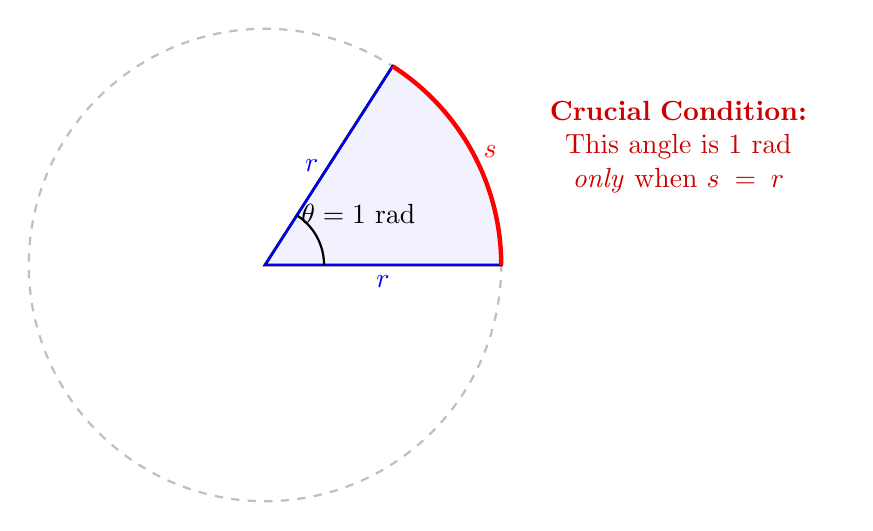
\begin{tikzpicture}[scale=1.5, line width=1pt]
        % Draw wedge
        \draw[thick, gray!50, dashed] (0,0) circle (2);
        
        % The pie slice
        \draw[fill=blue!5] (0,0) -- (0:2) arc (0:57.3:2) -- cycle;
        
        % Lines
        \draw[thick, blue] (0,0) -- (0:2) node[midway, below] {$r$};
        \draw[thick, blue] (0,0) -- (57.3:2) node[midway, left] {$r$};
        
        % The arc
        \draw[ultra thick, red] (0:2) arc (0:57.3:2) node[midway, right] {$s$};
        
        % The angle
        \draw[thick] (0.5,0) arc (0:57.3:0.5);
        \node at (28.6:0.9) {$\theta = 1 \text{ rad}$};
        
        % Annotation
        \node[text width=4cm, align=center, red!80!black] at (3.5, 1) {\textbf{Crucial Condition:}\\ This angle is 1 rad \emph{only} when $s = r$};
    \end{tikzpicture}
    \caption{The geometric definition of 1 radian.}
\end{figure}

\subsection{The Bridge Equation ($s = r\theta$)}
This definition gives us our first and most important formula linking the angular world to the linear world. If the angle $\theta$ is measured in radians, the actual distance traveled along the arc ($s$) is simply:
\begin{equation}
    s = r\theta
\end{equation}

\textbf{Converting Degrees to Radians:} \\
We know the circumference of a full circle is $s = 2\pi r$. Plugging this into our equation gives: 
\begin{equation*}
    2\pi r = r\theta \quad \Rightarrow \quad \theta = 2\pi \text{ rad}
\end{equation*}
Thus, $360^\circ = 2\pi \text{ rad}$, which gives the standard conversion: $180^\circ = \pi \text{ rad}$.

\subsection{Angular Displacement ($\Delta \theta$)}
In Grade 11, linear displacement ($\Delta \vec{d}$) was defined as a change in position. In rotational kinematics, we use \textbf{Angular Displacement ($\Delta \theta$)} to represent the angle an object rotates through.
\begin{equation}
    \Delta \theta = \theta_f - \theta_i
\end{equation}

\begin{itemize}
    \item Like linear displacement, it is a \textbf{vector} (it has direction).
    \item \textbf{Sign Convention:} By standard physics rules, \textbf{Counter-Clockwise (CCW)} is defined as positive ($+$), and \textbf{Clockwise (CW)} is negative ($-$).
\end{itemize}

\section{Angular Velocity and Acceleration}

With angular displacement defined, we can express how fast this angle changes.

\subsection{Angular Velocity ($\omega$)}
Angular velocity ($\omega$, the Greek letter omega) is the rate at which angular displacement changes over time.
\begin{equation}
  \omega = \frac{\Delta \theta}{\Delta t}
\end{equation}
\textit{Note: All points on a rigid rotating object (like a spinning merry-go-round) share the exact same $\omega$, no matter how far they are from the center.}

\subsection{Angular Acceleration ($\alpha$)}
Angular acceleration ($\alpha$, the Greek letter alpha) is the rate of change of angular velocity:
\begin{equation}
  \alpha = \frac{\Delta \omega}{\Delta t}
\end{equation}

\section{The Link Between Linear and Angular (Derivations)}

The primary advantage of using radians is that the linear distance $s$ (arc length) traveled by a particle is simply the product of the radius and the angular displacement ($s=r\theta$). 

If we observe the motion over a \textbf{very short time interval} ($\Delta t$), the change in arc length is directly proportional to the change in angle:
\begin{equation*}
    \Delta s = r (\Delta \theta)
\end{equation*}

By dividing both sides of this equation by the tiny time interval ($\Delta t$), we reveal a direct connection between the tangential speed $v$ and angular velocity $\omega$:

\begin{equation}
    \frac{\Delta s}{\Delta t} = r \left( \frac{\Delta \theta}{\Delta t} \right) \quad \Rightarrow \quad v = r\omega
\end{equation}

\textbf{Crucial Concept:} While $\Delta s / \Delta t$ mathematically gives an \emph{average} speed, if we imagine $\Delta t$ becoming infinitesimally small (approaching zero), it perfectly describes the \textbf{instantaneous} values precisely at a single geometric point. This is the foundational idea of Calculus!

Using the exact same algebraic trick over that extremely small $\Delta t$, substituting $v = r\omega$, we can connect tangential acceleration $a_t$ and angular acceleration $\alpha$:
\begin{equation}
    \frac{\Delta v}{\Delta t} = r \left( \frac{\Delta \omega}{\Delta t} \right) \quad \Rightarrow \quad a_t = r\alpha
\end{equation}

These relationships allow us to constantly switch between reading $v$ on a speedometer and calculating the $\omega$ of the spinning tires:

\begin{table}[h!]
\centering
\begin{tabular}{ll}
\toprule
\textbf{Angular Variable} & \textbf{Linear Counterpart (Translation)} \\ \midrule
Angular Displacement: $\theta$ & Arc Length (Distance): $s = r\theta$ \\
Angular Velocity: $\omega$ & Tangential Speed: $v = r\omega$ \\
Angular Acceleration: $\alpha$ & Tangential Acceleration: $a_t = r\alpha$ \\ \bottomrule
\end{tabular}
\end{table}

\subsection{Period ($T$) and Frequency ($f$)}
Before deriving centripetal acceleration, we must link $\omega$ to two macro-scale concepts:
\begin{itemize}
    \item \textbf{Period ($T$):} The time in seconds ($\text{s}$) to complete exactly \textbf{one full revolution} ($2\pi$ rads).
    \item \textbf{Frequency ($f$):} The number of full revolutions completed in \textbf{one second} ($\text{Hz}$ or $\text{s}^{-1}$).
\end{itemize}
They are reciprocals: $T = 1/f$. Therefore, the angular velocity can be directly calculated if we know how long one lap takes:
\begin{equation}
    \omega = \frac{\Delta \theta}{\Delta t} = \frac{2\pi}{T} = 2\pi f
\end{equation}

\section{Centripetal Acceleration ($a_c$) Derivation}

Unlike linear motion, an object in uniform circular motion is \textbf{always} accelerating, even if its speed $v$ is perfectly constant. Why? Because the \emph{direction} of the velocity vector is constantly changing. 

This center-seeking acceleration is called \textbf{centripetal acceleration} ($\vec{a}_c$). At any given moment, the velocity vector $\vec{v}$ is tangent to the circle, and the acceleration $\vec{a}_c$ points exactly to the center, meaning $\vec{v} \perp \vec{a}_c$.

\subsection{Geometric Proof Using Similar Triangles}
Consider an object moving from a generic point $A$ to point $B$ over a tiny time interval $\Delta t$. Its position vector sweeps out an angle $\Delta \theta$, and it travels an arc length roughly equal to a straight chord $\Delta s \approx v \Delta t$.

Meanwhile, the velocity vectors $\vec{v}_1$ and $\vec{v}_2$ (which are both of magnitude $v$) also rotate by that exact same angle $\Delta \theta$.

\begin{enumerate}
    \item \textbf{The Position Triangle:} Formed by radius $r$, radius $r$, and base chord $\Delta s$.
    \item \textbf{The Velocity Triangle:} Formed by the vectors $\vec{v}_1$, $\vec{v}_2$, and the difference vector $\Delta \vec{v}$.
    \item Because the central angle $\Delta \theta$ is identical in both, they are \textbf{similar isosceles triangles}.
\end{enumerate}

\begin{figure}[h]
    \centering
    \begin{minipage}{0.45\textwidth}
        \centering
        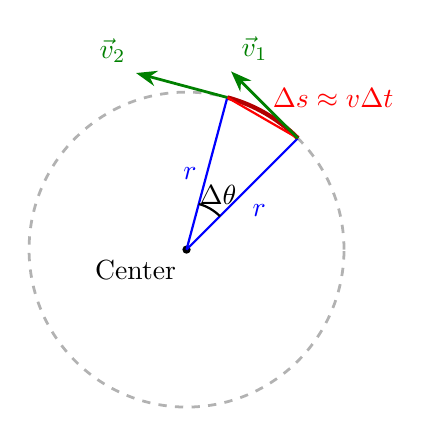
\begin{tikzpicture}[scale=1.0, line width=1pt]
            % Position Triangle embedded in a full circle
            \coordinate (O) at (0,0);
            
            % Draw the full reference circle
            \draw[dashed, gray!60] (O) circle (2);
            \fill (O) circle (1.5pt) node[below left] {Center};
            
            % Two coordinates on the circle
            \coordinate (A) at (75:2);
            \coordinate (B) at (45:2);
            
            % Emphasize the arc of travel
            \draw[ultra thick, red!70!black] (45:2) arc (45:75:2);
            
            % Draw the two radii
            \draw[thick, blue] (O) -- (A) node[midway, left] {$r$};
            \draw[thick, blue] (O) -- (B) node[midway, below right] {$r$};
            
            % Draw the chord \Delta s
            \draw[thick, red] (A) -- (B) node[midway, above right] {$\Delta s \approx v\Delta t$};
            
            % The angle \Delta \theta at the center
            \draw[thick] (45:0.6) arc (45:75:0.6);
            \node at (60:0.8) {$\Delta \theta$};
            
            % Show the tangent lines (velocities) originating from the circle
            % Object moves CCW from B (45 deg) to A (75 deg)
            \draw[-{Stealth[scale=1.0]}, green!50!black] (B) -- ++(135:1.2) node[above right] {$\vec{v}_1$};
            \draw[-{Stealth[scale=1.0]}, green!50!black] (A) -- ++(165:1.2) node[above left] {$\vec{v}_2$};
            
        \end{tikzpicture}
        
        \vspace{0.2cm}
        \small (a) The Position Triangle
    \end{minipage}%
    \hfill
    \begin{minipage}{0.45\textwidth}
        \centering
        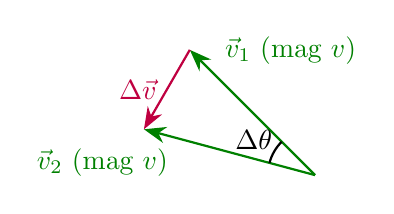
\begin{tikzpicture}[scale=1.5, line width=1pt]
            % Velocity Triangle
            \coordinate (O) at (0,0);
            
            % The v1 vector (matching tangency at B, 45+90 = 135 deg)
            \coordinate (V1) at (135:1.5);
            
            % The v2 vector (matching tangency at A, 75+90 = 165 deg)
            \coordinate (V2) at (165:1.5);
            
            % Draw the vectors
            \draw[-{Stealth[scale=1.2]}, thick, green!50!black] (O) -- (V1) node[pos=0.8, above right] {$\vec{v}_1$ (mag $v$)};
            \draw[-{Stealth[scale=1.2]}, thick, green!50!black] (O) -- (V2) node[pos=0.8, below left] {$\vec{v}_2$ (mag $v$)};
            
            % Draw the Delta V vector from V1 to V2
            \draw[-{Stealth[scale=1.2]}, thick, purple] (V1) -- (V2) node[midway, left] {$\Delta \vec{v}$};
            
            % The angle \Delta \theta
            \draw[thick] (135:0.4) arc (135:165:0.4);
            \node at (150:0.6) {$\Delta \theta$};
            
        \end{tikzpicture}
        
        \vspace{0.2cm}
        \small (b) The Velocity Triangle ($\Delta \vec{v} = \vec{v}_2 - \vec{v}_1$)
    \end{minipage}
    \caption{Visualizing the Similar Triangles: Since both sets of vectors sweep through the exact same angle $\Delta \theta$, the physical position triangle is geometrically similar to the velocity vector triangle.}
\end{figure}

By setting up the ratio of corresponding sides from these similar triangles:
\begin{equation}
    \frac{\Delta v}{v} = \frac{\Delta s}{r}
\end{equation}

Since we know $\Delta s = (v)(\Delta t)$, we can substitute it in:
\begin{equation*}
    \frac{\Delta v}{v} = \frac{v \Delta t}{r}
\end{equation*}

Divide both sides by $\Delta t$ to isolate $\frac{\Delta v}{\Delta t}$ (which is exactly the definition of acceleration $\vec{a}_c$):
\begin{equation*}
    a_c = \frac{\Delta v}{\Delta t} = \frac{v \cdot v}{r}
\end{equation*}

This elegantly gives us the holy grail equation for the \emph{magnitude} of circular motion:
\begin{equation}
    a_c = \frac{v^2}{r}
\end{equation}

\textbf{What about the direction?} 
Look closely at the Velocity Triangle in Figure (b). The purple vector $\Delta \vec{v}$ (which dictates the direction of our acceleration $\vec{a}_c$) generally points inward. Imagine making the time interval $\Delta t$ infinitesimally small. As the angle $\Delta \theta$ shrinks to nearly zero, the base of this skinny isosceles triangle ($\Delta \vec{v}$) becomes exactly perpendicular ($90^\circ$) to the two velocity vectors. Since the velocity is tangent to the circle edge, a vector exactly perpendicular to the tangent must point \textbf{directly toward the center} of the circle. This explicit visual proof is exactly why it is named \textbf{centripetal} (``center-seeking'') acceleration.

\subsection{Alternative Forms Using $\omega$ and $T$}
By substituting our bridge equation ($v = r\omega$) into the holy grail equation, we get the rotational version:
\begin{equation}
    a_c = \frac{(r\omega)^2}{r} = \omega^2 r
\end{equation}

And by substituting $\omega = 2\pi/T$, we can find the acceleration strictly from the radius and the period:
\begin{equation}
    a_c = (\frac{2\pi}{T})^2 r = \frac{4\pi^2 r}{T^2}
\end{equation}

\vspace{0.5cm}

\begin{figure}[h]
    \centering
    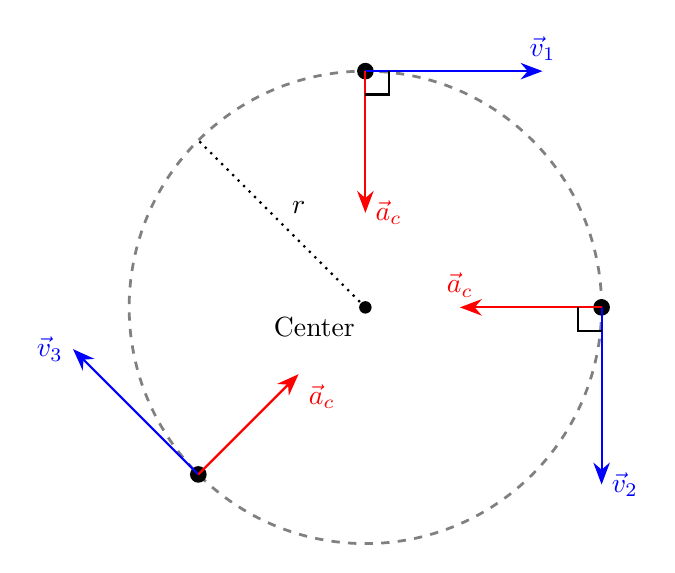
\begin{tikzpicture}[scale=1.5, line width=1pt]
        % The circular path
        \draw[dashed, gray] (0,0) circle (2);
        \fill (0,0) circle (1.5pt) node[below left] {Center};
        
        % Point 1 (Top)
        \fill (0,2) circle (2pt);
        \draw[-{Stealth[scale=1.2]}, blue, thick] (0,2) -- (1.5,2) node[above] {$\vec{v}_1$};
        \draw[-{Stealth[scale=1.2]}, red, thick] (0,2) -- (0,0.8) node[right] {$\vec{a}_c$};
        % Right angle marker
        \draw (0.2,2) -- (0.2, 1.8) -- (0, 1.8);
        
        % Point 2 (Right)
        \fill (2,0) circle (2pt);
        \draw[-{Stealth[scale=1.2]}, blue, thick] (2,0) -- (2,-1.5) node[right] {$\vec{v}_2$};
        \draw[-{Stealth[scale=1.2]}, red, thick] (2,0) -- (0.8,0) node[above] {$\vec{a}_c$};
        % Right angle marker
        \draw (2,-0.2) -- (1.8, -0.2) -- (1.8, 0);

        % Point 3 (Bottom Left angle, 225 degrees)
        \coordinate (P3) at (225:2);
        \fill (P3) circle (2pt);
        \draw[-{Stealth[scale=1.2]}, blue, thick] (P3) -- ++(-45:-1.5) node[left] {$\vec{v}_3$};
        \draw[-{Stealth[scale=1.2]}, red, thick] (P3) -- ++(45:1.2) node[below right] {$\vec{a}_c$};
        
        % Radius line
        \draw[dotted, thick] (0,0) -- (135:2) node[midway, above right] {$r$};
    \end{tikzpicture}
    \caption{In Uniform Circular Motion, velocity $\vec{v}$ is always tangent, and acceleration $\vec{a}_c$ always points to the center. Thus, $\vec{v} \perp \vec{a}_c$.}
\end{figure}

\newpage

\section{Total Acceleration (Non-Uniform Circular Motion)}

So far, we have largely focused on \textbf{Uniform Circular Motion (UCM)}, where the object's speed $v$ remains perfectly constant. In this scenario, the \emph{only} acceleration present is the center-seeking centripetal acceleration ($\vec{a}_c = v^2/r$) responsible for changing the direction.

But what if a car is driving in a circle \emph{and} stepping on the gas pedal at the same time? 

In this case, the object is undergoing \textbf{Non-Uniform Circular Motion}. We must deal with two independent components of acceleration simultaneously:
\begin{itemize}
    \item \textbf{Centripetal Acceleration ($\vec{a}_c$):} Changes the \emph{direction}. It always points towards the center of the circle.
    \item \textbf{Tangential Acceleration ($\vec{a}_t$):} Changes the \emph{speed} (magnitude of velocity). It is always tangent to the circle (parallel to $\vec{v}$). From our bridge equations, $a_t = r\alpha$.
\end{itemize}

Since these two vectors are always perfectly perpendicular ($\vec{a}_c \perp \vec{a}_t$), we can find the \textbf{Total Acceleration ($\vec{a}_{\text{tot}}$)} using the Pythagorean theorem and simple trigonometry:

\begin{equation}
    a_{\text{tot}} = \sqrt{a_c^2 + a_t^2}
\end{equation}

\vspace{0.5cm}

\begin{figure}[h]
    \centering
    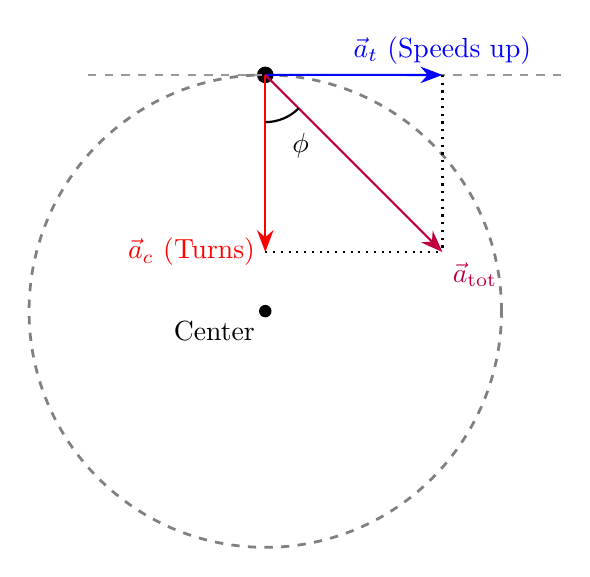
\begin{tikzpicture}[scale=1.5, line width=1pt]
        % The circular path
        \draw[dashed, gray] (0,0) circle (2);
        \fill (0,0) circle (1.5pt) node[below left] {Center};
        
        % The Point
        \coordinate (P) at (0,2);
        \fill (P) circle (2pt);
        
        % Tangential Velocity / Acceleration Line
        \draw[dashed, gray!80] (-1.5, 2) -- (2.5, 2);
        
        % The Vectors
        \draw[-{Stealth[scale=1.2]}, blue, thick] (P) -- (1.5,2) node[above] {$\vec{a}_t$ (Speeds up)};
        \draw[-{Stealth[scale=1.2]}, red, thick] (P) -- (0,0.5) node[left] {$\vec{a}_c$ (Turns)};
        
        % The Total Acceleration Vector
        \draw[-{Stealth[scale=1.2]}, thick, purple] (P) -- (1.5,0.5) node[below right] {$\vec{a}_{\text{tot}}$};
        
        % Vector Addition Parallelogram
        \draw[dotted, thick] (1.5,2) -- (1.5,0.5);
        \draw[dotted, thick] (0,0.5) -- (1.5,0.5);
        
        % Angle Phi
        \draw[thick] (0, 1.6) arc (270:315:0.4);
        \node at (0.3, 1.4) {$\phi$};
        
    \end{tikzpicture}
    \caption{In Non-Uniform Circular Motion, the total acceleration $\vec{a}_{\text{tot}}$ is the vector sum of both the centripetal and tangential accelerations.}
\end{figure}

The angle $\phi$ that the total acceleration makes with the radial direction (pointing to the center) can be found using the inverse tangent function:
\begin{equation}
    \phi = \tan^{-1}\left(\frac{a_t}{a_c}\right)
\end{equation}

This concludes the complete kinematic picture of an object moving in a circle, whether its speed is steady or changing!

\end{document}
